\documentclass[../../../../main.tex]{subfiles}
\begin{document}

図のような立体 $ABCD-EFGH$ がある．
上底面 $ABCD$，下底面 $EFGH$ はともに正方形であって，
両底面はたがいに平行であり，
4つの側面 $ABFE$，$BCGF$，$CDHG$，$DAEH$ は台形であって，
$AE=BF=CG=DH$ である．
また下底面の1辺の長さは12，両底面の間の距離は4である．

上底面の1辺の長さが $x$ のとき，
側面 $ABFE$ の面積を $S(x)$ とする．
$x$ が $2 \leqq x \leqq 10$ の範囲を動くときの $S(x)$ の最大値と最小値を求めよ．

\begin{figure}[htbp]
  \centering
  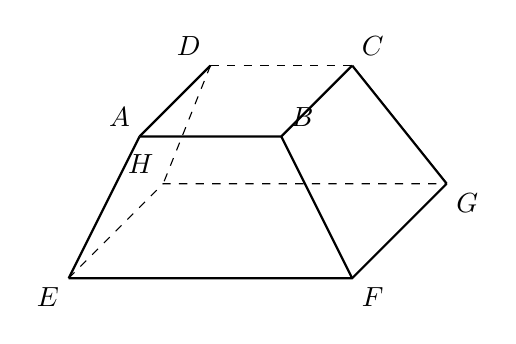
\begin{tikzpicture}[scale=1.5]
    \coordinate (A) at (-0.6, 1.2);
    \coordinate (B) at (0.6, 1.2);
    \coordinate (C) at (1.2, 1.8);
    \coordinate (D) at (0.0, 1.8);

    \coordinate (E) at (-1.2, 0);
    \coordinate (F) at (1.2, 0);
    \coordinate (G) at (2.0, 0.8);
    \coordinate (H) at (-0.4, 0.8);

    \draw[dashed] (E) -- (H) -- (G);
    \draw[dashed] (D) -- (H);
    \draw[dashed] (D) -- (C);

    \draw[thick] (A) -- (B) -- (C);
    \draw[thick] (A) -- (D);
    \draw[thick] (E) -- (F) -- (G);
    \draw[thick] (A) -- (E);
    \draw[thick] (B) -- (F);
    \draw[thick] (C) -- (G);

    \node[above left] at (A) {$A$};
    \node[above right] at (B) {$B$};
    \node[above right] at (C) {$C$};
    \node[above left] at (D) {$D$};
    \node[below left] at (E) {$E$};
    \node[below right] at (F) {$F$};
    \node[below right] at (G) {$G$};
    \node[above left] at (H) {$H$};
  \end{tikzpicture}
\end{figure}

\end{document}
